\section{General setup}\label{sec:general-setup}
GRATiS uses GROOVE as a replacement of the STS in ATM. Figure~\ref{fig:tooling} shows this graphically. GROOVE has several exploration strategies for exploring a graph grammar to a GTS. GRATiS has a new strategy, the \textit{symbolic exploration strategy}, which transforms the graph grammar to an STS instead. The interface on the GROOVE side is implemented by means of a \textit{remote exploration strategy}. This strategy uses the symbolic exploration strategy to derive an STS and sends the STS formatted as JSON to the ATM interface. The ATM interface parses the JSON to an STS, starts the STS Engine with the STS and initiates the test run.

\begin{figure}[ht]
  \begin{center}
    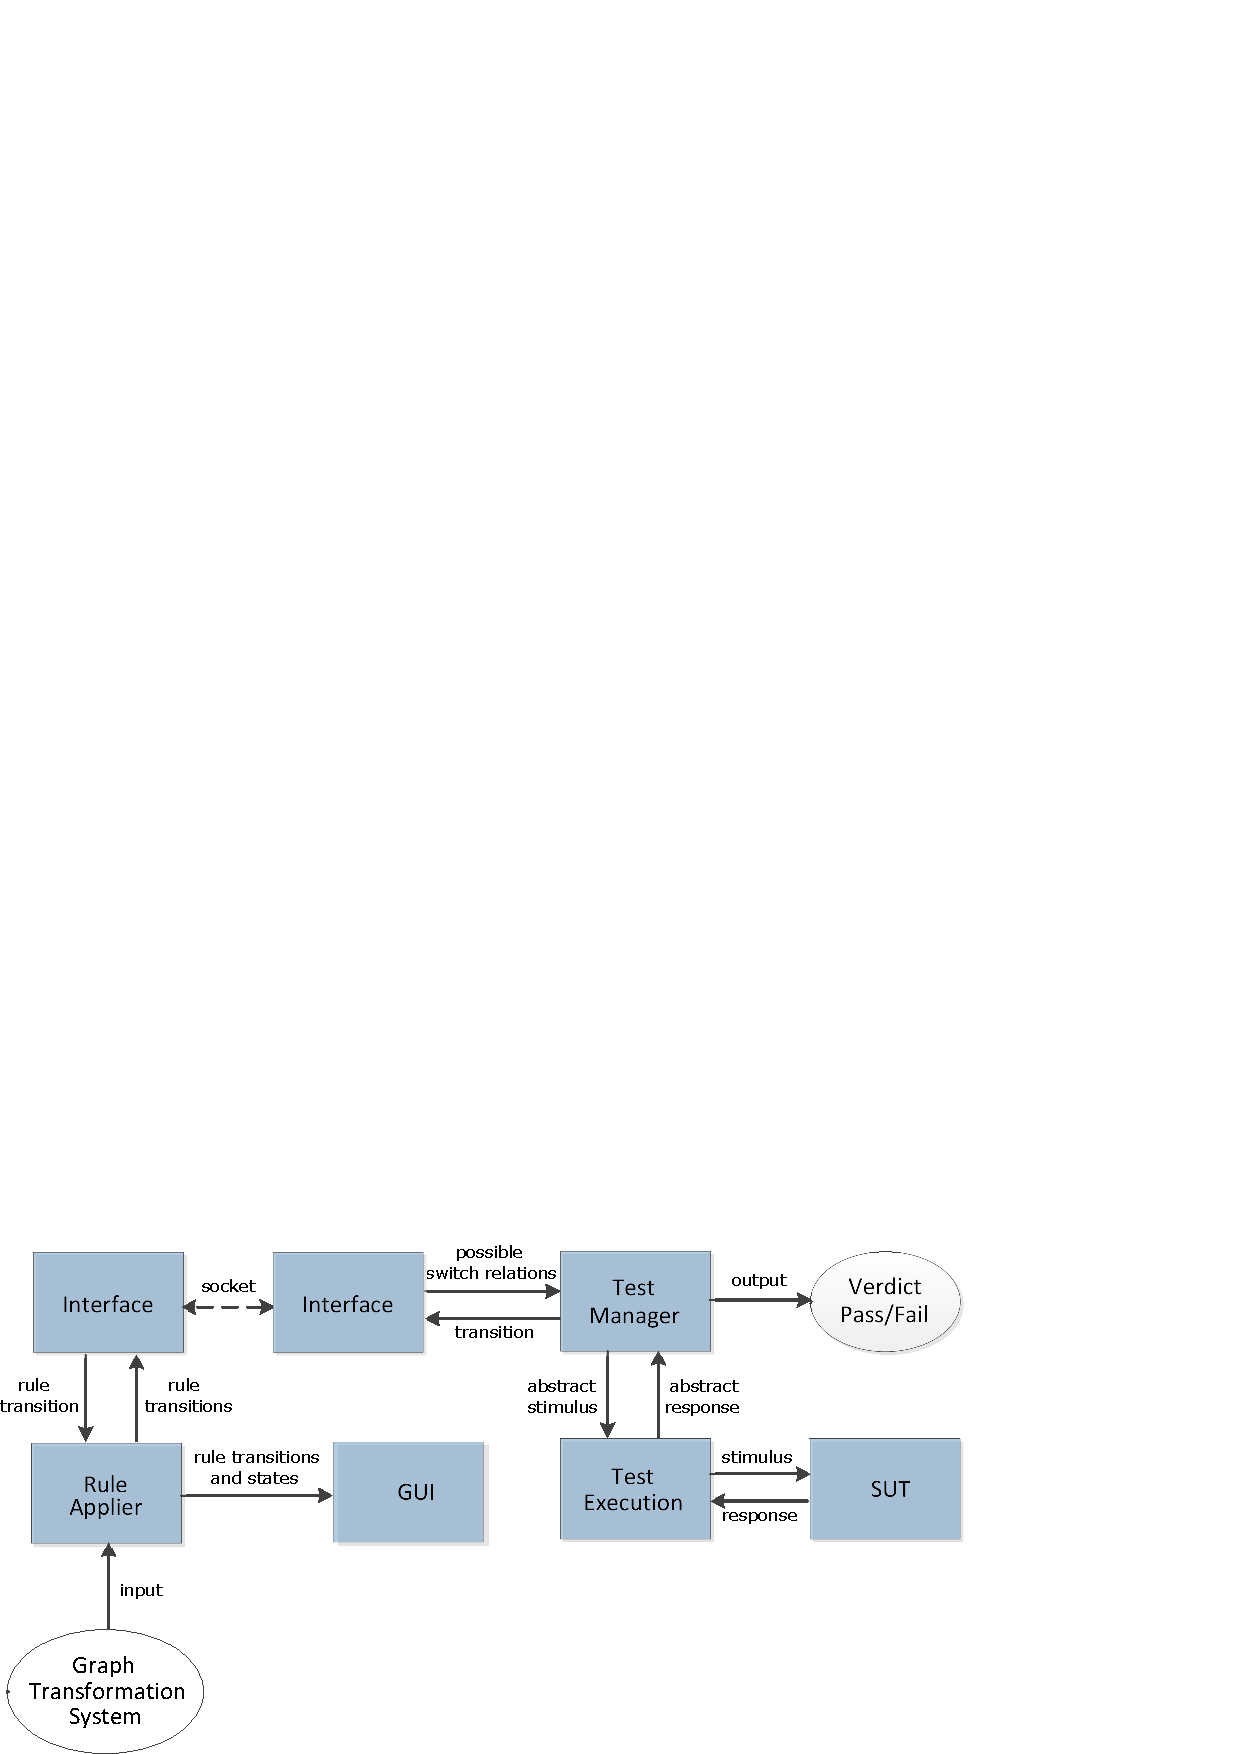
\includegraphics[width=\textwidth]{tooling.pdf}
  \end{center}
  \caption{The GRATiS design: replacing the STS with GROOVE}
  \label{fig:tooling}
\end{figure}

\section{Offline vs. on-the-fly model exploration}\label{sec:offline-on-the-fly}
The exploration of a graph grammar can be done in two ways: \textit{on the fly}, rule transitions are explored only when chosen by ATM, or \textit{offline}, the graph grammar is first fully transformed to an STS and then sent to ATM.

On-the-fly model exploration works well on large and even infinite models. However, coverage statistics cannot be calculated on GRATiS, if the model exploration is done on the fly. The number of states/locations and transitions/switch relations the model has when completely explored are not known, so a percentage cannot be derived. As coverage statistics are an important metric, the offline model exploration is chosen for GRATiS.


